\section{Equivalent Intermediate Formulation} \label{EqIntFor} Our focus is now on modifying the methodology of Section \ref{Conservative} to make better approximations of \eqref{GP_counterparts_finite}. This section presents an enhanced formulation of \eqref{GP_safe_convex} that is equivalent to the robust counterparts in \eqref{GP_counterparts_finite} but with smaller, easier to handle posynomial constraints.

In order to divide the posynomial into smaller posynomials, consider the set $\mathbf{I}_i = \left\{ 1,2,...,K_i\right\} $ associated with the $i^{th}$ constraint, and define the equivalence relation $\mathcal{R}$ (see Appendix \ref{EqRel} for the definition of an equivalence relation) given by
\begin{equation}
\begin{aligned}
\mathcal{R} = \{&k_1 \sim k_2 \iff e^{\vec{a_{ik_1}}\left(\zeta\right)\vec{x} + b_{ik_1}\left(\zeta\right)} \text{ and } e^{\vec{a_{ik_2}}\left(\zeta\right)\vec{x} + b_{ik_2}\left(\zeta\right)} \text{ are dependent} \}
\end{aligned}
\label{equivalence_relation}
\end{equation}

$\mathcal{R}$ splits $\mathbf{I}_i$ into equivalence classes $S_{i,1},\ S_{i,2},\ ...\ S_{i,N_e^i}$, $N_e^i \leq K_i$. Because these classes are completely independent it must be the case that
$$
\max_{\vec{\zeta} \in \mathcal{Z}} \left\{\textstyle{\sum}_{k=1}^{K_i}e^{\vec{a_{ik}}\left(\zeta\right)\vec{x} + b_{ik}\left(\zeta\right)}\right\} = \textstyle{\sum}_{j=1}^{N_e^i} {\displaystyle \max_{\vec{\zeta} \in \mathcal{Z}}} \left\{\textstyle{\sum}_{k \in S_{i,j}}e^{\vec{a_{ik}}\left(\zeta\right)\vec{x} + b_{ik}\left(\zeta\right)}\right\}
$$

%This suggests that the robust constraints with $N_e^i > 1$ could be made smaller by adding some dummy variables.
The robust counterparts of \eqref{GP_counterparts_finite} are thus equivalent to
\begin{equation}
\begin{aligned}
&\min &&f_0(x)\\
&\text{s.t.} &&\textstyle{\sum}_{j=1}^{N_e^i} e^{t_{ij}} &&\leq 1 \qquad &&\forall i \in 1,...,m\\
& &&\max_{\vec{\zeta} \in \mathcal{Z}} \left\{\textstyle{\sum}_{k \in S_{i,j}} e^{\vec{a_{ik}}\left(\zeta\right)\vec{x} + b_{ik}\left(\zeta\right)} \right\} &&\leq e^{t_{ij}} &&\forall i \in 1,...,m\\
& && && &&\forall j \in 1, ..., N_e^i\\
\end{aligned}
\label{equivalent_class_setP}
\end{equation}

Our main concern is now the larger posynomials, which motivate the introduction of a \textbf{categorized form} of a robust GP, in which constraints are categorized into three sets. The set of monomial constraints is labeled by $\mathbf{M} \equiv \left\{(i, j): |S_{i,j}| = 1\right\}$, two-term posynomials by $\mathbf{N} \equiv \left\{(i, j): |S_{i,j}| = 2\right\}$, and constraints with three or more posynomials are labeled by $\mathbf{P} \ \equiv \left\{(i,j): |S_{i,j}| \geq 3\right\}$. Further definining $S_{i,j}^k$ as the $k^{th}$ element of $S_{i,j}$, the \textbf{categorized form} is
\begin{equation}
\begin{aligned}
&\min &\multicolumn{2}{l}{$f_0(x)$}\\
&\text{s.t.} &\multicolumn{2}{l}{$\textstyle{\sum}_{j=1}^{N_e^i} e^{t_{ij}}$} &&\leq 1 \qquad &&\forall i \in 1,...,m\\
& &\max_{\vec{\zeta} \in \mathcal{Z}}& \left\{\textstyle{\sum}_{k \in S_{i,j}} e^{\vec{a_{ik}}\left(\zeta\right)\vec{x} + b_{ik}\left(\zeta\right)} \right\} &&\leq e^{t_{ij}} &&\forall(i,j) \in \mathbf{P}\\
& &\max_{\vec{\zeta} \in \mathcal{Z}}&
\multicolumn{5}{l}{$\left\{e^{\vec{a_{iS_{i,j}^1}}\left(\zeta\right)\vec{x} + b_{iS_{i,j}^1}\left(\zeta\right)} + e^{\vec{a_{iS_{i,j}^2}}\left(\zeta\right)\vec{x} + b_{iS_{i,j}^2}\left(\zeta\right)} \right\} \leq e^{t_{ij}}$}\\
&&&&& &&\forall(i,j) \in \mathbf{N}\\
& &\max_{\vec{\zeta} \in \mathcal{Z}}& \left\{e^{\vec{a_{iS_{i,j}^1}}\left(\zeta\right)\vec{x} + b_{iS_{i,j}^1}\left(\zeta\right)} \right\} &&\leq e^{t_{ij}} &&\forall(i,j) \in \mathbf{M}\\
\end{aligned}
\label{categorizedForm}
\end{equation}
Figure \ref{partitioning} presents an illustrative example of this partitioning. 
\begin{figure}[H]
\captionsetup{justification=centering, font=small}
\begin{center}
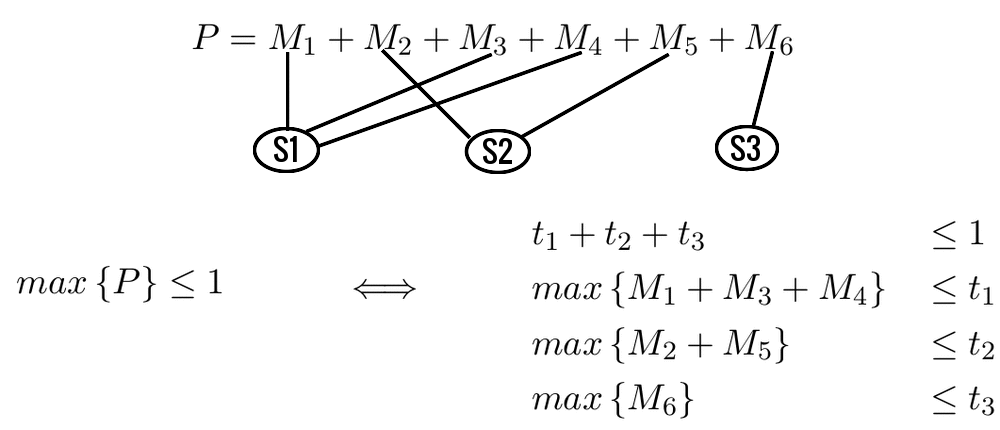
\includegraphics[scale=0.25]{partitioning.png}
\end{center}
\caption{Example of partitioning a large posynomial into smaller posynomials.}
\label{partitioning}
\end{figure}

This partitioning will not be of much benefit when all monomials in a posynomial are uncertain and dependent on each other. However, when most monomials are certain, or when some are independent, a large posynomial can be effectively reduced into several smaller ones, or even into monomials. In practice, most GPs for engineering design are only sparsely dependent, and so this formulation provides a significant decrease (often by more than half) in the number of constraints.